% ===== Setup Font =====
\usepackage[sfdefault,lf]{carlito}
\usepackage[T1]{fontenc}
\renewcommand*\oldstylenums[1]{\carlitoOsF #1}

% ==== Import Math Packages =====
\usepackage{amsmath, amssymb, amsthm}
\usepackage{mathtools}

% ==== Import Plotting Packages =====
\usepackage{tikz}
\usepackage{pgfplots}
\pgfplotsset{compat=1.18}
\usepgfplotslibrary{fillbetween}
\usetikzlibrary{decorations.pathreplacing,calligraphy}
\usepackage{pgffor}
\usepgfplotslibrary{colorbrewer}
\usetikzlibrary{pgfplots.colorbrewer}

% ==== Import Styling Packages =====
\usepackage{enumitem}
\usepackage[pages=some, placement=bottom]{background}
\usepackage{moresize}
\usepackage{relsize}
\usepackage{hyperref}
\hypersetup{colorlinks=true,allcolors=blue}
\usepackage{hypcap}
\usepackage{verbatim}

% ==== Theorem =====
\newtheorem*{theorem*}{Teorema}

% ===== Cover Setup =====
\backgroundsetup{
scale=1,
color=black,
opacity=1,
angle=0,
contents={%
  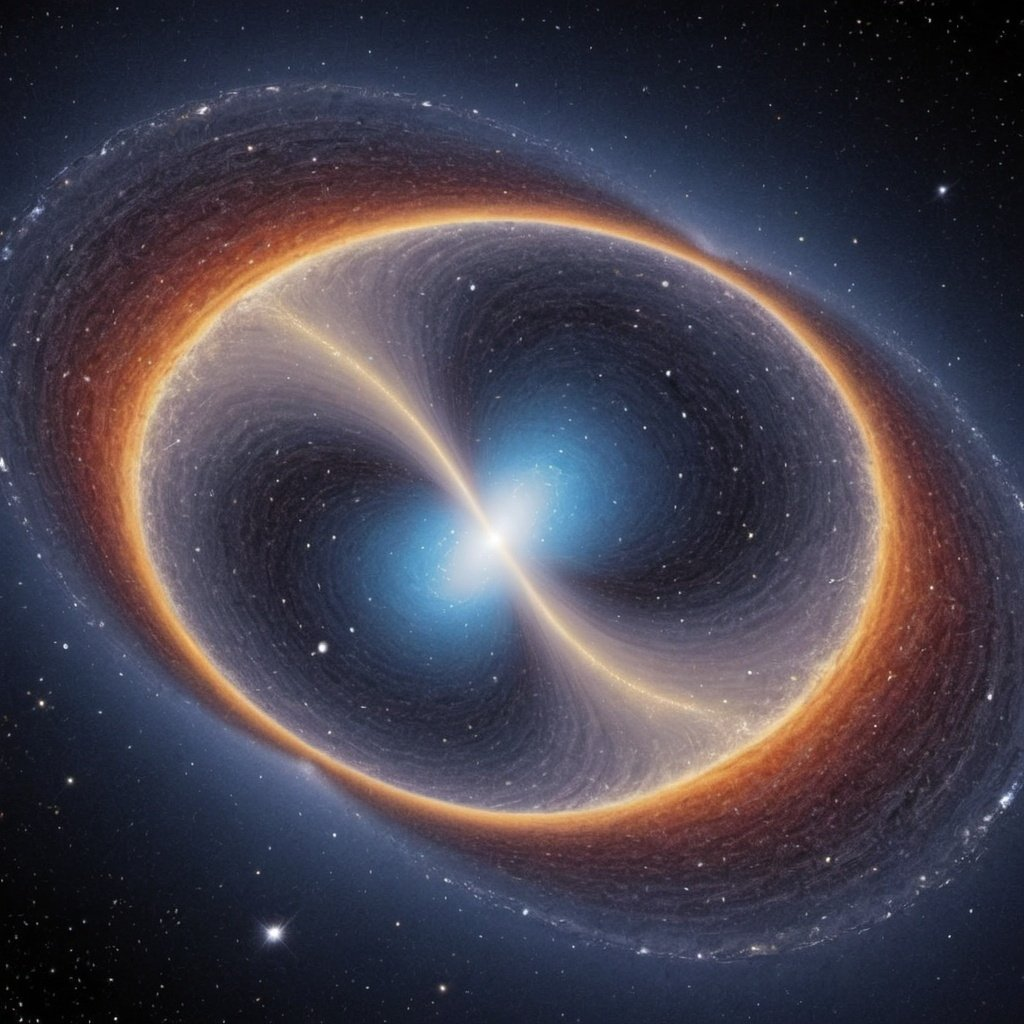
\includegraphics[width=\paperwidth,height=0.8\paperheight]{cover_kalkulus 1.png}
  }%
}

% ==== Custom Declarations =====
\DeclarePairedDelimiter\abs{\lvert}{\rvert}
\DeclarePairedDelimiter\floor{\lfloor}{\rfloor}
\DeclarePairedDelimiter\cic{[ }{] }
\DeclarePairedDelimiter\oic{( }{] }
\DeclarePairedDelimiter\cio{[ }{) }
\DeclarePairedDelimiter\oio{( }{) }
\DeclarePairedDelimiter\set{\{ }{\} }
\DeclarePairedDelimiter\brk{(}{)}
\newcommand{\drv}[2]{\frac{d}{d#1}\brk*{#2}}
\newcommand{\drvL}[2]{D_{#1}\brk*{#2}}
\newcommand{\ds}{\displaystyle}
\newcommand{\eval}[3]{\left.\brk*{#1}\right\rvert_{#2}^{#3}}

% ==== Reuseable Figures =====
% Point
\newcommand{\point}[2]{
	\node [draw, shape = circle, fill=#1, minimum size = 0.1cm, inner sep=0pt] 
        at #2 {}
}
% Real Line
\newcommand{\realline}{
	\draw[stealth-stealth] (-5,0) node[below]{$-\infty$}--(5,0) node[below]{$\infty$}
}